\begin{figure*}[!t]
    \centering
    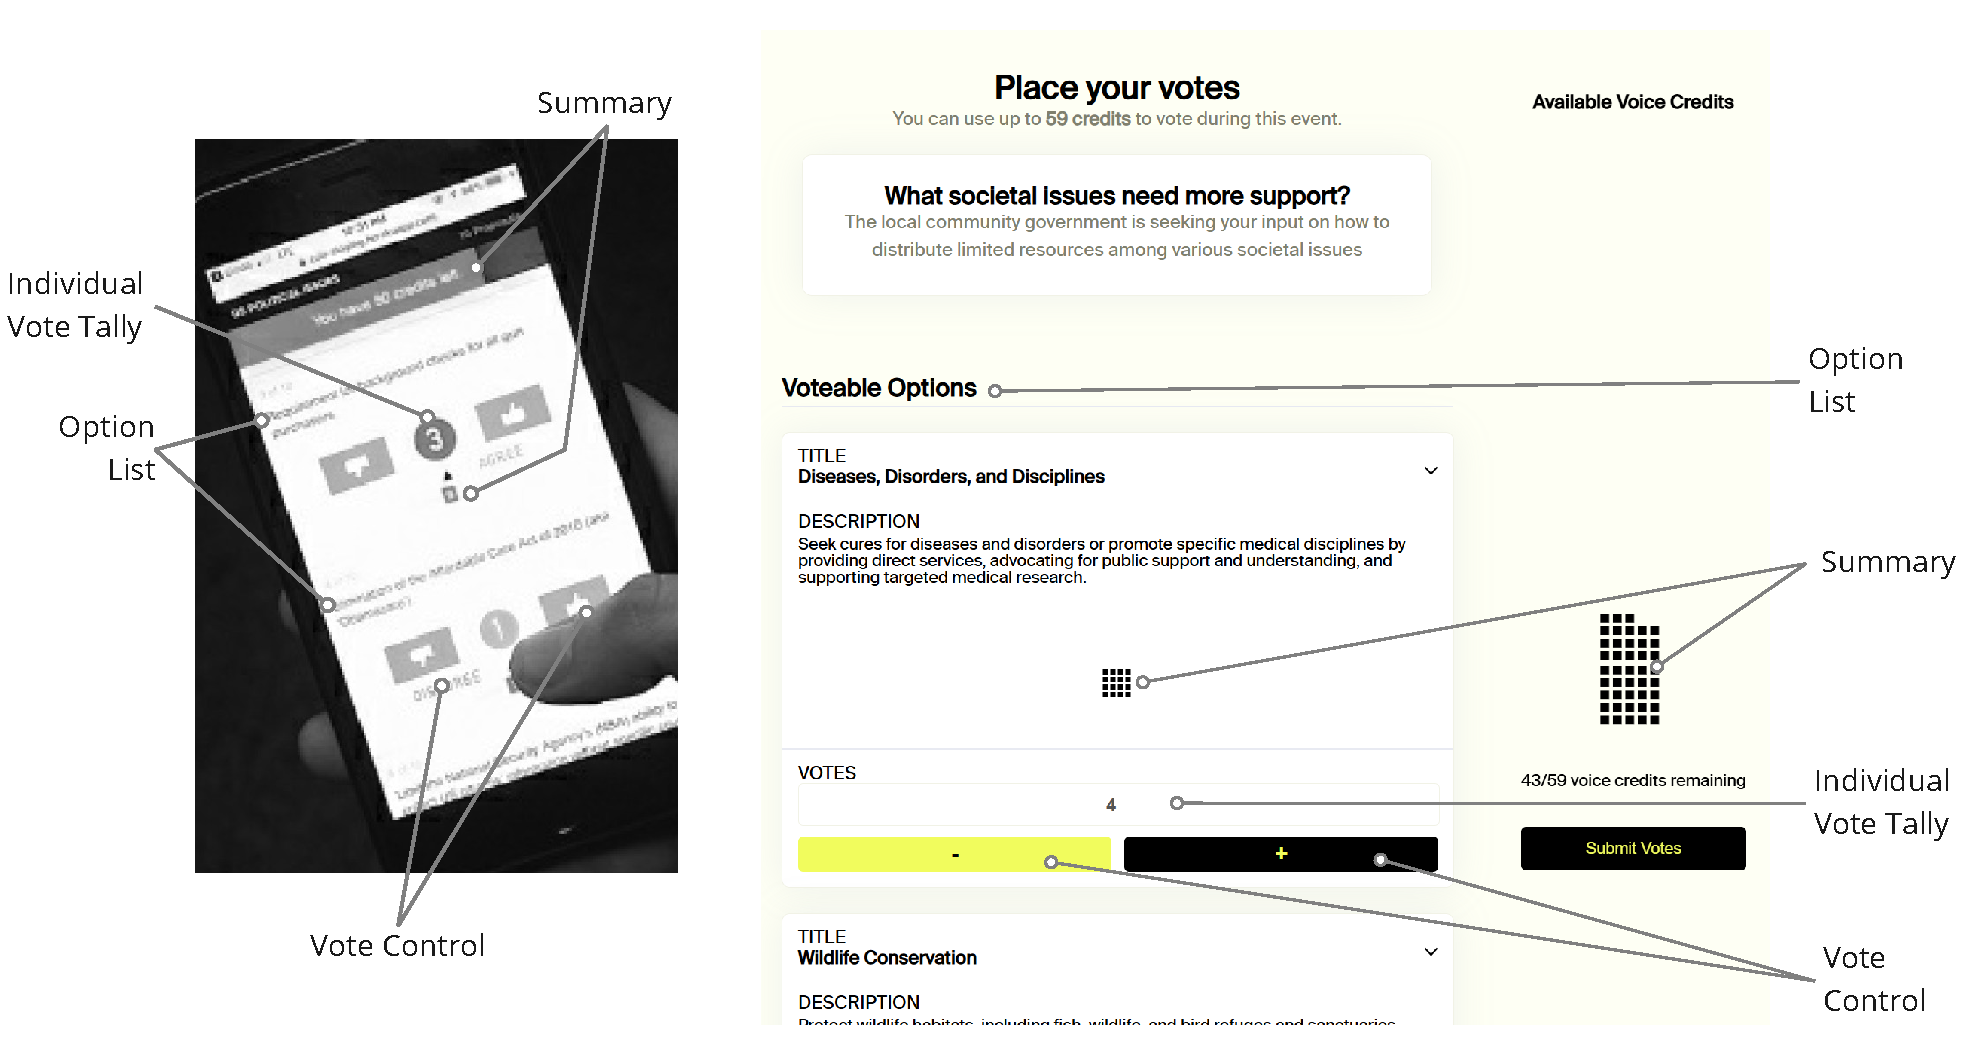
\includegraphics[width=0.85\textwidth]{content/image/curr_interface/recent_annotated.pdf}
    \caption{A selection of two QV interfaces. The interface on the left was used in the first empirical QV research~\cite{quarfoot2017quadratic}. Little information is available about the software, except for an image from~\citet{posner2018radical}. The interface on the right is an open-sourced QV interface~\cite{RadicalxChangeQuadraticvoting2024} forked from GitCoin~\cite{gitcoinReadWhitepaperGitcoin}, used by the RadicalxChange community~\cite{radicalxchange}. Both interfaces share the common elements with different visual representations.}
    \Description{There are two smaller figures in this figure. On the left is a black and white image of a mobile phone displaying a voting interface from software by WeDesign, used in empirical QV research. A hand holds the phone, and the screen shows a prompt related to background checks for gun purchases. There are thumbs-up and thumbs-down icons labeled "Agree" and "Disagree," with numbers indicating the current number of votes (e.g., 3 votes for "Agree"). A remaining vote budget is displayed at the top as a progress bar, indicating "50 choices left." The user is interacting with the interface, selecting either agree or disagree on the prompts. On the right is A screenshot of a QV interface designed for voting on societal issues that need more support. The screen displays two options: "Diseases, Disorders, and Disciplines" and "Wildlife Conservation," with a brief description under each. Users can adjust votes with plus and minus buttons, and the current vote count (e.g., 3 votes for Diseases, -2 votes for Wildlife Conservation) is displayed. The total available credits are shown on the right side as a grid of small blocks, with 46 out of 59 credits remaining. There is also a "Submit Votes" button. A menu on the left allows users to jump to different societal issues. Both images are annotated to locate the elements described in the main text.}
    \label{fig:rcx_interface_annotated}
\end{figure*}